%%
%%  Department of Electrical, Electronic and Computer Engineering.
%%  EPR400/2 Final Report - Technical Documentation.
%%  Copyright (C) 2011-2021 University of Pretoria.
%%

\section{HARDWARE part of the project}

\subsection{Record 1. System block diagram}

\ldots

\newpage

\subsection{Record 2.  Systems level description of the design}

\ldots

\newpage

\subsection{Record 3. Complete circuit diagrams and description}

See next page for complete schematic of the robotic embedded controller circuit schematic that was created during the PCB design process.

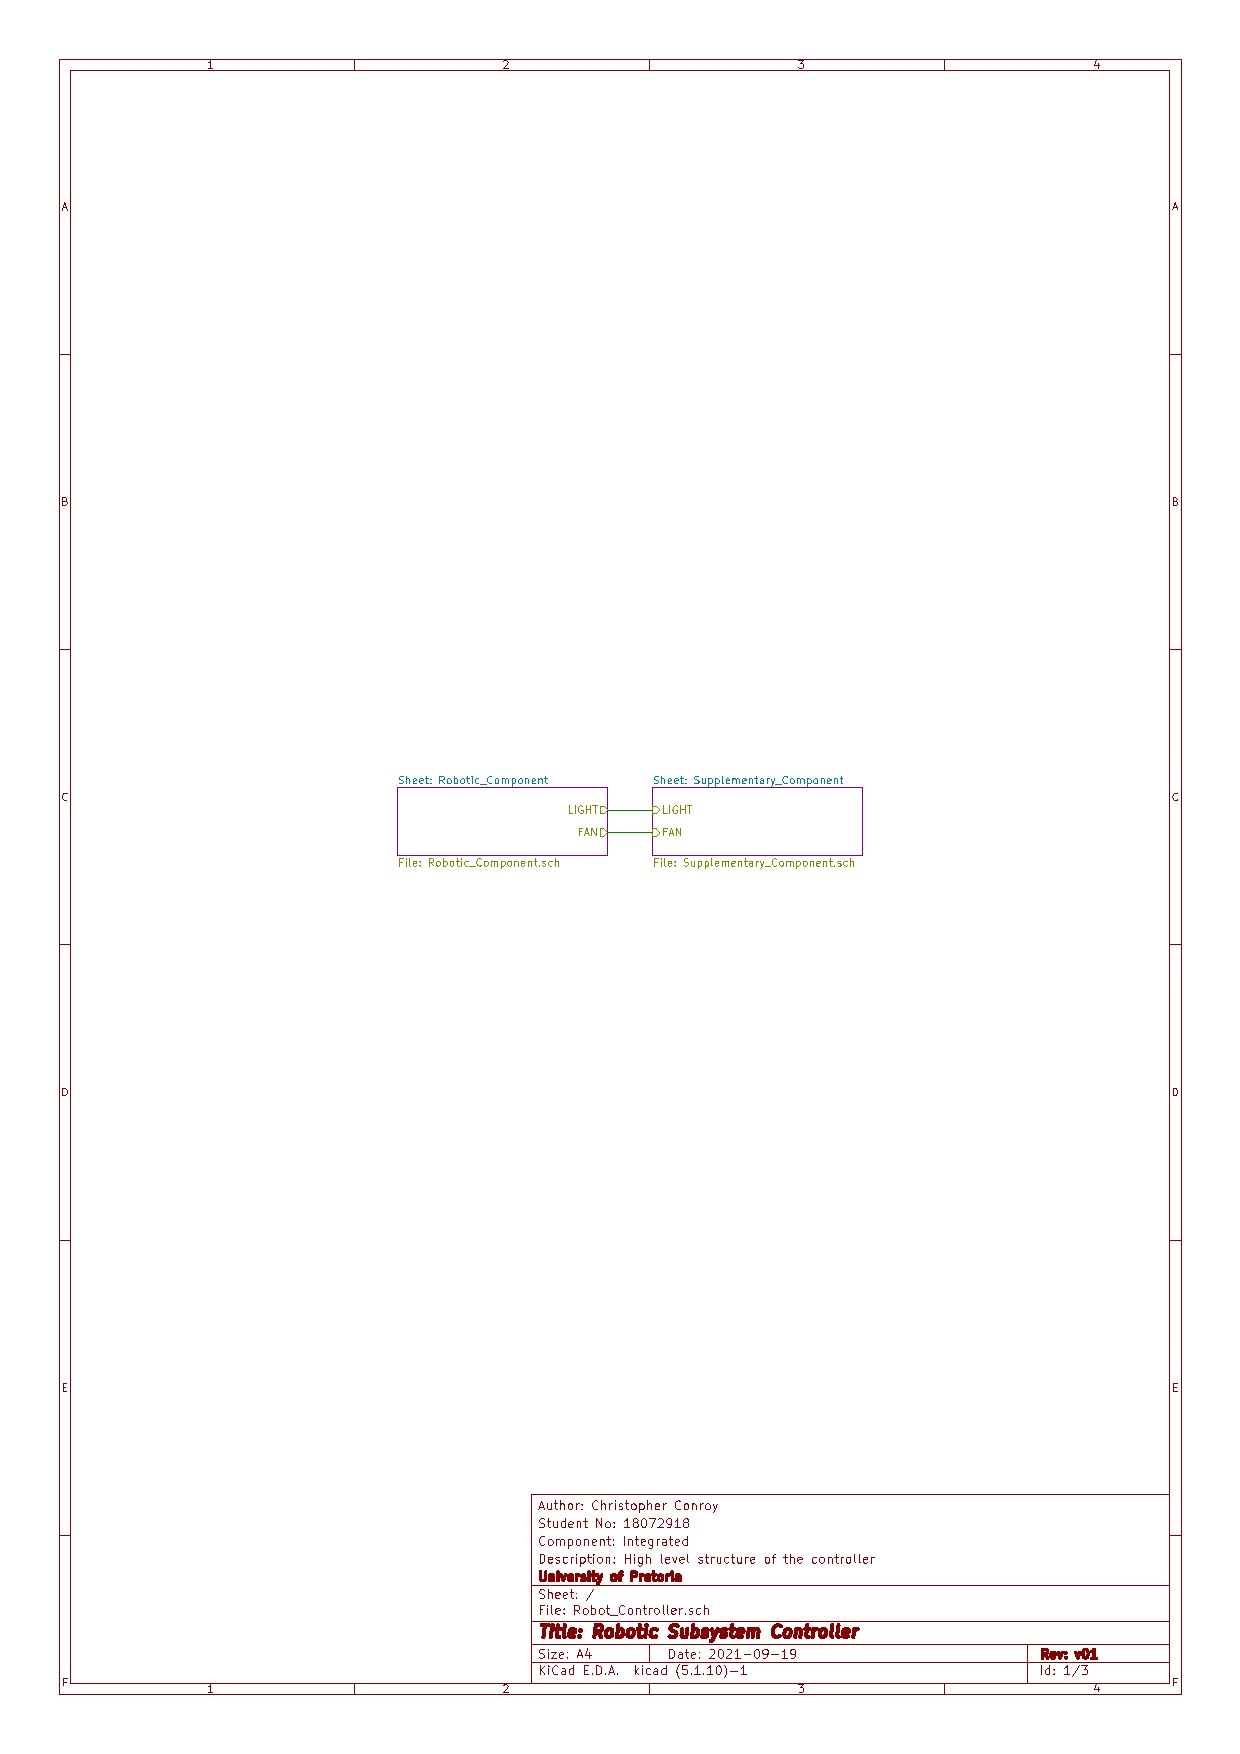
\includepdf[pages=-]{pdfs/electrical-design.pdf}

\subsection{Record 4. Hardware acceptance test procedure}

\ldots

\newpage

\subsection{Record 5. User guide}

\ldots

\newpage

%% --------------------------------------------------------------------

\section{SOFTWARE part of the project}

\subsection{Record 6. Software process flow diagrams}

\ldots

\newpage

\subsection{Record 7. Explanation of software modules}

\ldots

\newpage

\subsection{Record 8. Complete source code}
Complete code has been submitted separately on the AMS.

\newpage

\subsection{Record 9. Software acceptance test procedure}

\ldots

\newpage

\subsection{Record 10. Software user guide}

\ldots

\newpage

%% --------------------------------------------------------------------

\section{EXPERIMENTAL DATA}

\subsection{Record 11. Experimental data}

\subsubsecnonumhidden{Qualification Test 1 Results}

\ldots

\subsubsecnonumhidden{Qualification Test 3 Results}

\ldots

\subsubsecnonumhidden{Qualification Test 4 Results}

\begin{table}[H]
	\renewcommand{\arraystretch}{1.3}
	\centering
	\begin{tabular}{|>{\raggedright}m{1.5cm}|>{\raggedright}m{1.9cm}|>{\raggedright}m{1.9cm}|>{\raggedright}m{1.9cm}|>{\raggedright}m{1.8cm}|>{\raggedright}m{1.6cm}|>{\raggedright\arraybackslash}m{1.6cm}|}
		\hline
		\textbf{Sample Set} & \textbf{X Position (steps)} & \textbf{Y Position (steps)} & \textbf{Z Position (steps)} & \textbf{Reference Length (pixels)} & \textbf{X Points Range (pixels)} & \textbf{Y Points Range (pixels)} \\
		\hline
		1 & 0    & 0    & 0 & 79,168 & 9,751  & 8,03   \\
		\hline
		2 & 0    & 1125 & 0 & 61,265 & 13,883 & 11,059 \\
		\hline
		3 & 507  & 562  & 0 & 70,112 & 15,882 & 12,176 \\
		\hline
		4 & 1015 & 0    & 0 & 75,279 & 15,853 & 12,257 \\
		\hline
		5 & 1015 & 1125 & 0 & 72,198 & 11,063 & 8,388 \\
		\hline
	\end{tabular}
	\caption{\label{tab:techdoc-qtp4-xy1}Pixel measurements using the point cluster images for the x- and y-axis repeatability test.}
\end{table}

\begin{table}[H]
	\renewcommand{\arraystretch}{1.3}
	\centering
	\begin{tabular}{|>{\raggedright}m{2.5cm}|>{\raggedright}m{4cm}|>{\raggedright\arraybackslash}m{4cm}|}
		\hline
		\textbf{Sample Set} & \textbf{X Points Range (mm)} & \textbf{Y Points Range (mm)} \\
		\hline
		1 & 0,2463 & 0,2028  \\ 
		\hline
		2 & 0,4532 & 0,3610 \\ 
		\hline
		3 & 0,4530 & 0,3473  \\ 
		\hline
		4 & 0,4211 & 0,3256 \\
		 \hline
		5 & 0,3064 & 0,2323 \\ 
		\hline
	\end{tabular}
	\caption{\label{tab:techdoc-qtp4-xy2}X- and y-axis repeatability test measurements after conversion from pixel units in Table \ref{tab:techdoc-qtp4-xy1}.}
\end{table}

\begin{table}[H]
	\renewcommand{\arraystretch}{1.3}
	\centering
	\begin{tabular}{|>{\raggedright}m{1.5cm}|>{\raggedright}m{1.9cm}|>{\raggedright}m{1.9cm}|>{\raggedright}m{1.9cm}|>{\raggedright}m{1.8cm}|>{\raggedright}m{1.6cm}|>{\raggedright\arraybackslash}m{1.6cm}|}
		\hline
		\textbf{Sample Set} & \textbf{X Position (steps)} & \textbf{Y Position (steps)} & \textbf{Z Position (steps)} & \textbf{Reference Length (pixels)} & \textbf{Z Points Range (pixels)} & \textbf{Z Points Range (mm)} \\
		\hline
		1 & 852 & 70  & 500  & 60,001 & 23     & 0,7666 \\ \hline
		2 & 852 & 70  & 2300 & 61,26  & 19,96  & 0,6516 \\ \hline
		3 & 502 & 400 & 500  & 60,962 & 18,506 & 0,6071 \\ \hline
		4 & 502 & 400 & 2300 & 60,705 & 15,173 & 0,4998 \\ \hline
		5 & 194 & 700 & 500  & 60,397 & 17,557 & 0,5813 \\ \hline
		6 & 194 & 700 & 2300 & 60,27  & 19     & 0,6304 \\ \hline
	\end{tabular}
	\caption{\label{tab:techdoc-qtp4-z1}Pixel measurements using the point cluster images for the z-axis repeatability test.}
\end{table}

\subsubsecnonumhidden{Qualification Test 5 Results}

\begin{table}[H]
	\renewcommand{\arraystretch}{1.3}
	\centering
	\begin{tabular}{|>{\raggedright}m{1.5cm}|>{\raggedright}m{2.5cm}|>{\raggedright}m{2.5cm}|>{\raggedright\arraybackslash}m{3cm}|}
		\hline
		\textbf{Sample} & \textbf{$y_0$ Deviation $\delta_0$ (mm)} & \textbf{$y_1$ Deviation $\delta_1$ (mm)} & \textbf{Deviation Angle $\phi$ ($\degree$)} \\
		\hline
		1  & 0,64  & -0,66 & 0,3146  \\ \hline
		2  & -0,36 & 0,53  & -0,2154 \\ \hline
		3  & -0,11 & 0,2   & -0,0750  \\ \hline
		4  & 0,32  & -0,22 & 0,1307  \\ \hline
		5  & 0,12  & -0,08 & 0,0484 \\ \hline
		6  & 1,51  & -1,85 & 0,8132 \\ \hline
		7  & -0,16 & 0,32  & -0,1161 \\ \hline
		8  & 0,7   & -0,47 & 0,2831 \\ \hline
		9  & -1,24 & 1,01  & -0,5445 \\ \hline
		10 & -1,43 & 1,22  & -0,6414 \\ \hline
		11 & 1,12  & -0,31 & 0,3461 \\ \hline
		12 & 0,66  & -0,84 & 0,3630  \\ \hline
		13 & 0,98  & -1,18 & 0,5228  \\ \hline
		14 & -0,36 & 0,53  & -0,2154 \\ \hline
		15 & 0,23  & -0,44 & 0,1621  \\ \hline
		16 & 0,6   & -0,95 & 0,3751 \\ \hline
		17 & -0,47 & 0,66  & -0,2735 \\ \hline
		18 & 0,57  & -0,4  & 0,2347  \\ \hline
	\end{tabular}
	\caption{\label{tab:techdoc-qtp5-z-rot1}Deviation measurements of drawn cube orientation lines and the calculated angle of deviation of the line cube.}
\end{table}

\subsubsecnonumhidden{Qualification Test 6 Results}

\begin{table}[H]
	\renewcommand{\arraystretch}{1.3}
	\centering
	\begin{tabular}{|>{\raggedright}m{1.4cm}|>{\raggedright}m{1.8cm}|>{\raggedright}m{1.8cm}|>{\raggedright}m{1.8cm}|>{\raggedright}m{1.8cm}|>{\raggedright}m{1.8cm}|>{\raggedright\arraybackslash}m{1.8cm}|}
		\hline
		\textbf{Set Sample} & \textbf{True X Position (steps)} & \textbf{True Y Position (steps)} & \textbf{True Angle ($\degree$)} & \textbf{Detected X Position (steps)} & \textbf{Detected Y Position (steps)} & \textbf{Detected Angle ($\degree$)} \\
		\hline
		1  & 2   & 20   & 0 & 3   & 23   & -0,26 \\ \hline
		2  & 347 & 20   & 0 & 347 & 26   & -1,23 \\ \hline
		3  & 681 & 21   & 0 & 678 & 25   & 0,46  \\ \hline
		4  & 986 & 22   & 0 & 982 & 26   & 0,5   \\ \hline
		5  & 4   & 369  & 0 & 6   & 371  & 2,39  \\ \hline
		6  & 344 & 369  & 0 & 346 & 372  & 0,45  \\ \hline
		7  & 680 & 369  & 0 & 676 & 373  & 1,2   \\ \hline
		8  & 984 & 370  & 0 & 980 & 372  & 0     \\ \hline
		9  & 18  & 720  & 0 & 20  & 719  & 1,4   \\ \hline
		10 & 347 & 719  & 0 & 348 & 718  & 0,49  \\ \hline
		11 & 663 & 720  & 0 & 658 & 719  & 2,35  \\ \hline
		12 & 988 & 719  & 0 & 983 & 720  & 0,51  \\ \hline
		13 & 14  & 1079 & 0 & 14  & 1077 & 0,72  \\ \hline
		14 & 356 & 1080 & 0 & 355 & 1077 & 1,2   \\ \hline
		15 & 679 & 1080 & 0 & 677 & 1078 & 0,49  \\ \hline
		16 & 989 & 1081 & 0 & 987 & 1080 & 1,22  \\ \hline
	\end{tabular}
	\caption{\label{tab:techdoc-qtp6-set1}True poses of the first test set of cubes for qualification test 6 along with the corresponding estimated poses detected by the \textit{Vision System}.}
\end{table}

\begin{table}[H]
	\renewcommand{\arraystretch}{1.3}
	\centering
	\begin{tabular}{|>{\raggedright}m{1.4cm}|>{\raggedright}m{1.8cm}|>{\raggedright}m{1.8cm}|>{\raggedright}m{1.8cm}|>{\raggedright}m{1.8cm}|>{\raggedright}m{1.8cm}|>{\raggedright\arraybackslash}m{1.8cm}|}
		\hline
		\textbf{Set Sample} & \textbf{True X Position (steps)} & \textbf{True Y Position (steps)} & \textbf{True Angle ($\degree$)} & \textbf{Detected X Position (steps)} & \textbf{Detected Y Position (steps)} & \textbf{Detected Angle ($\degree$)} \\
		\hline
		1  & 83  & 77   & 45 & 85  & 80   & -44,98 \\ \hline
		2  & 396 & 61   & 45 & 395 & 65   & 44,31  \\ \hline
		3  & 677 & 77   & 45 & 673 & 82   & 44,66  \\ \hline
		4  & 974 & 54   & 45 & 971 & 59   & 41,5   \\ \hline
		5  & 214 & 245  & 45 & 214 & 246  & -44,68 \\ \hline
		6  & 505 & 252  & 45 & 504 & 524  & 44,65  \\ \hline
		7  & 777 & 286  & 45 & 772 & 289  & -44,62 \\ \hline
		8  & 19  & 438  & 45 & 22  & 439  & -44,66 \\ \hline
		9  & 307 & 450  & 45 & 308 & 450  & -43,96 \\ \hline
		10 & 530 & 533  & 45 & 527 & 532  & 44,07  \\ \hline
		11 & 916 & 447  & 45 & 909 & 449  & -43    \\ \hline
		12 & 26  & 733  & 45 & 27  & 732  & -44,65 \\ \hline
		13 & 271 & 790  & 45 & 271 & 788  & 43,31  \\ \hline
		14 & 654 & 711  & 45 & 650 & 709  & 45     \\ \hline
		15 & 928 & 733  & 45 & 923 & 731  & -43,66 \\ \hline
		16 & 25  & 1038 & 45 & 25  & 1035 & 44,66  \\ \hline
		17 & 358 & 1012 & 45 & 358 & 1009 & -44,67 \\ \hline
		18 & 625 & 1041 & 45 & 621 & 1037 & -44,66 \\ \hline
		19 & 937 & 1028 & 45 & 933 & 1025 & -42,27 \\ \hline
	\end{tabular}
	\caption{\label{tab:techdoc-qtp6-set2}True poses of the second test set of cubes for qualification test 6 along with the corresponding estimated poses detected by the \textit{Vision System}.}
\end{table}

\begin{figure}[!ht]
	\centering
	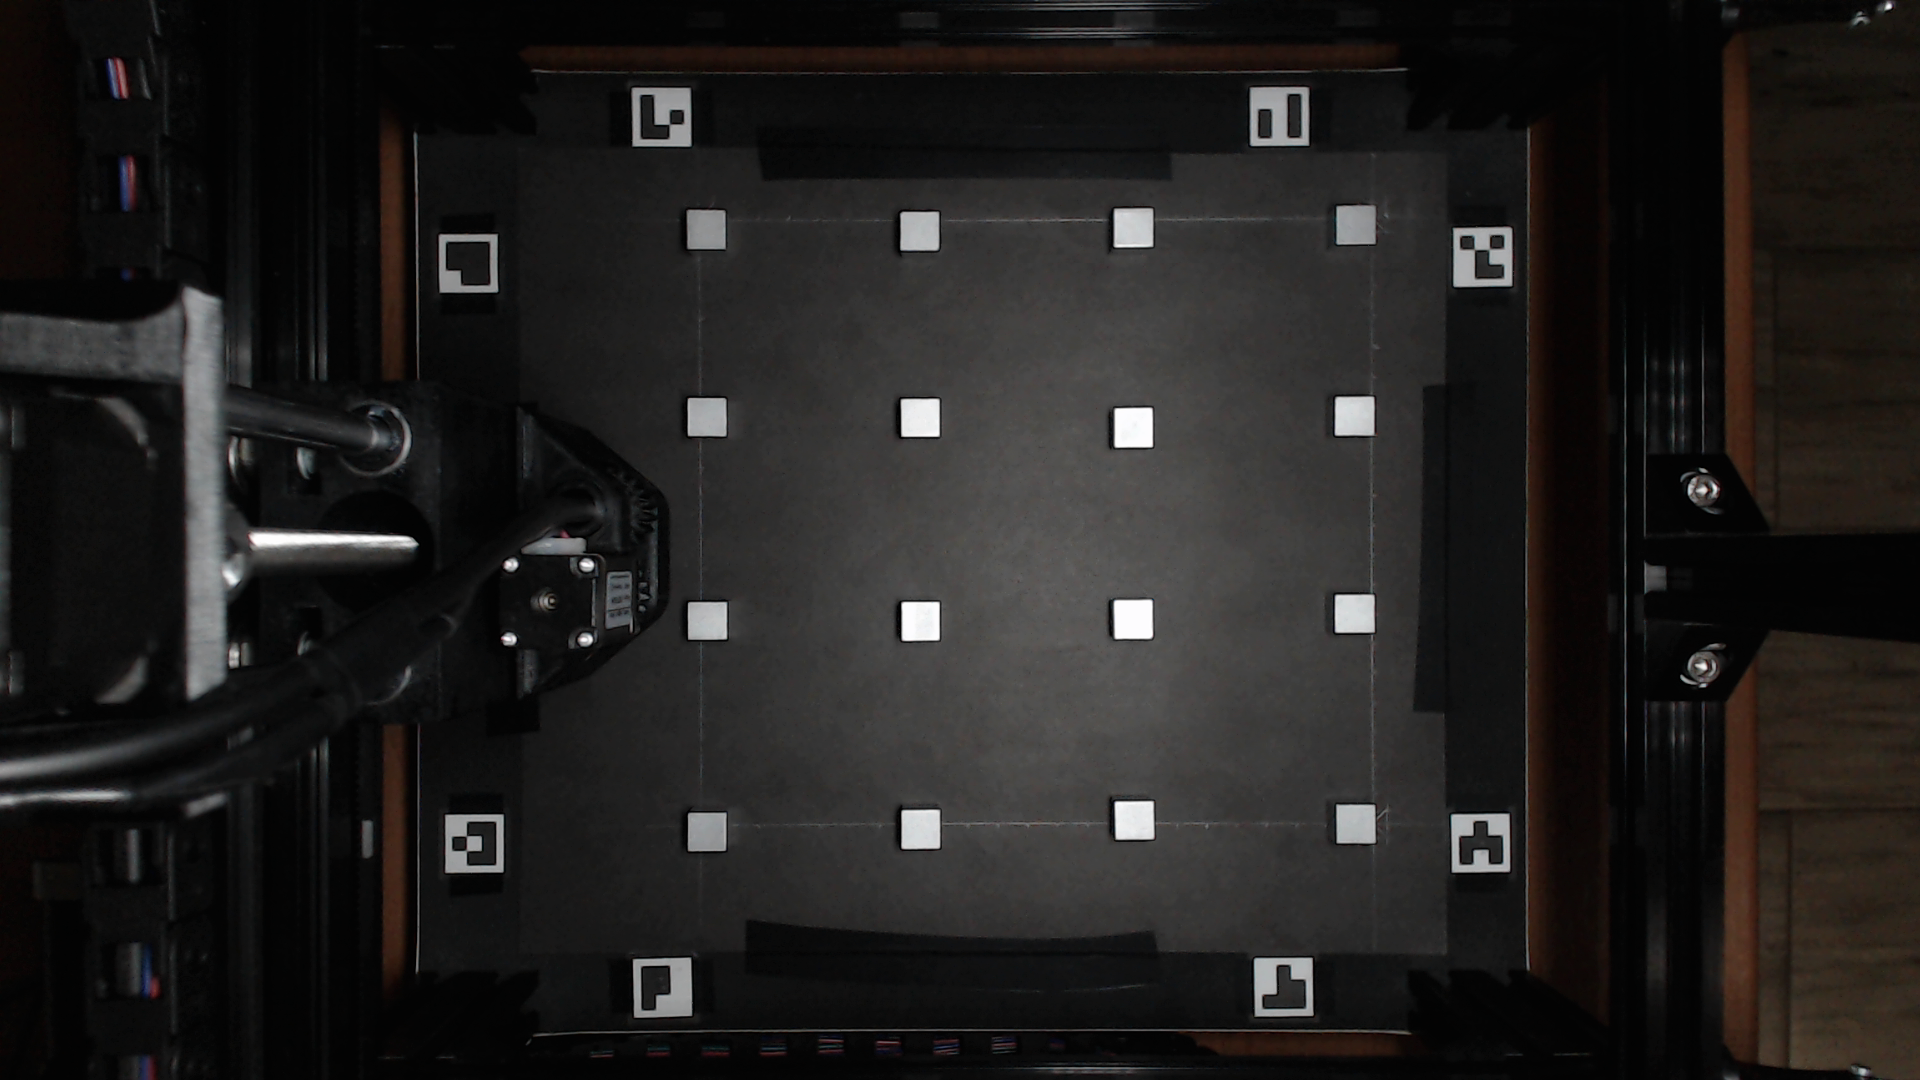
\includegraphics[width=1\linewidth]{figures/qtp6-set1.png}
	\caption{First test set of known cube positions and orientations (0$\degree$) in the robot's workspace for qualification test 6.}
	\label{fig:qtp6-set1}
\end{figure}

\begin{figure}[!ht]
	\centering
	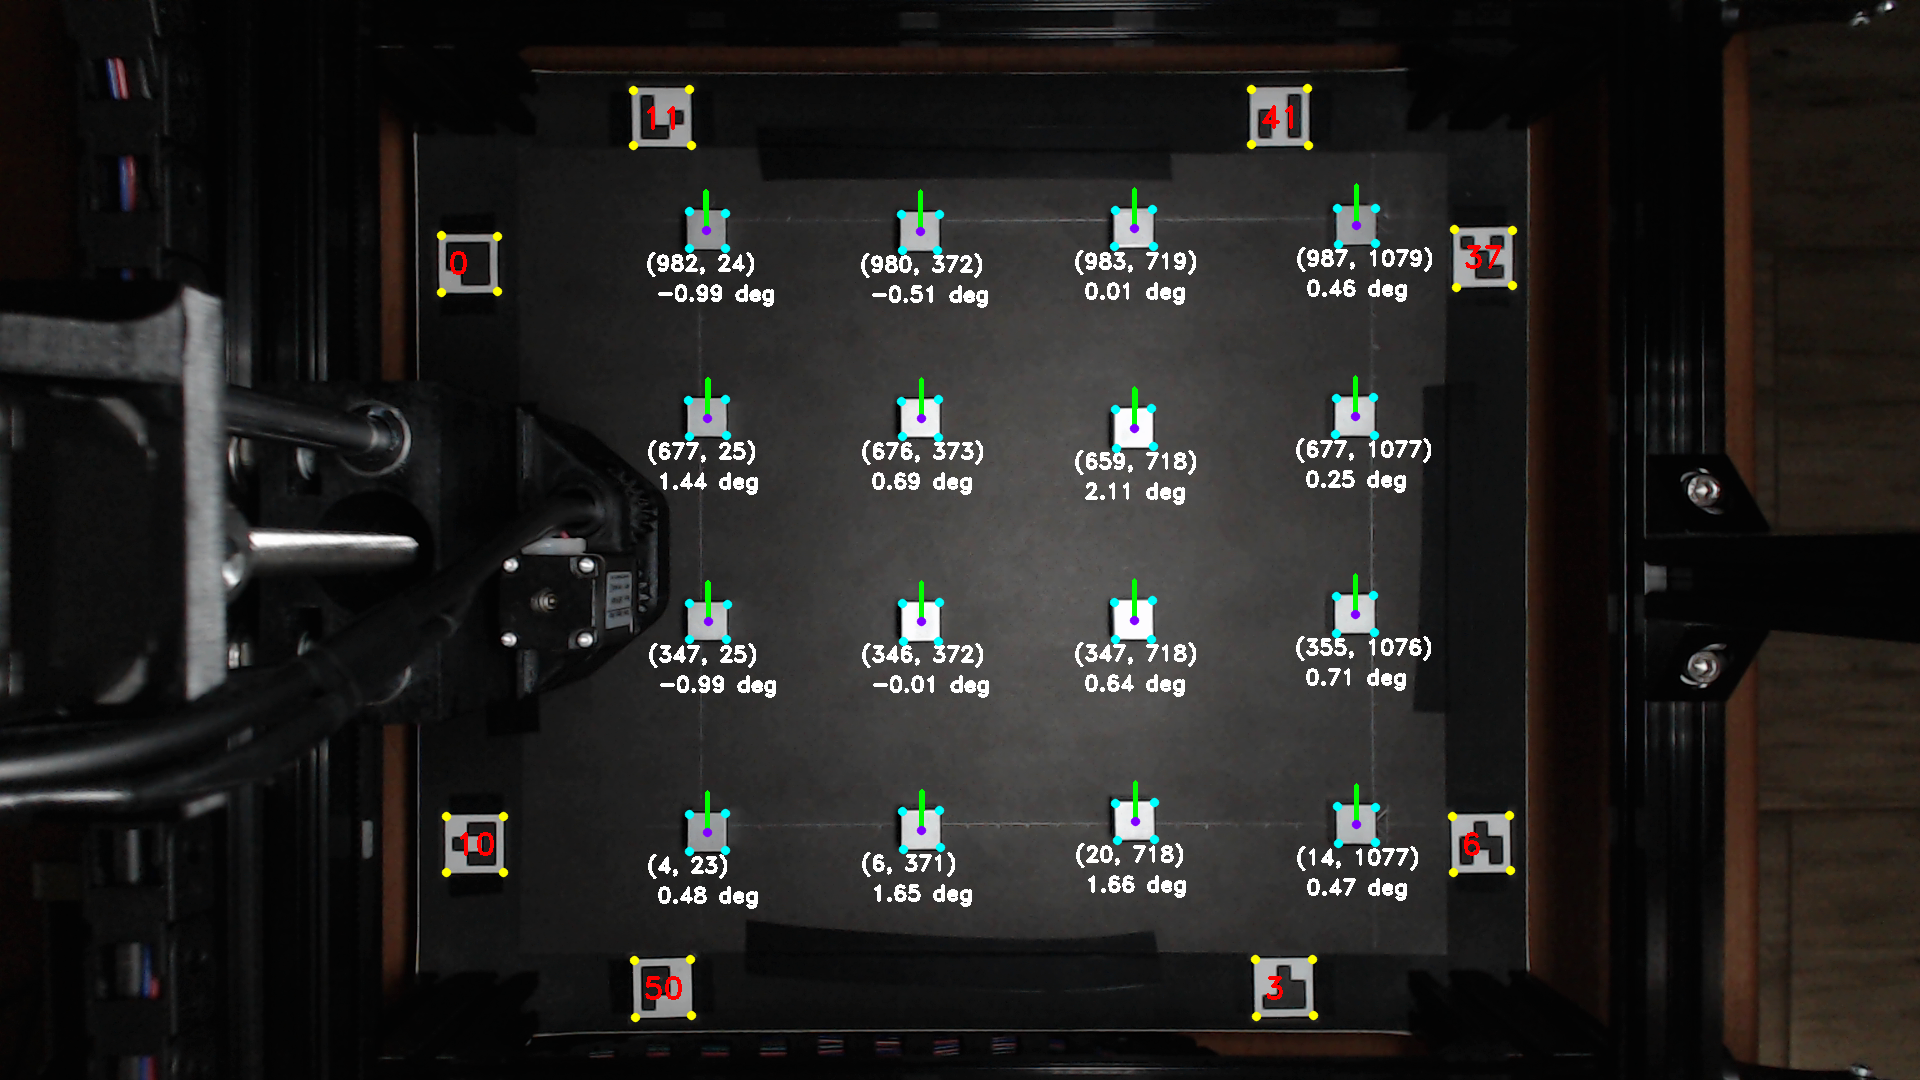
\includegraphics[width=1\linewidth]{figures/qtp6-set1-annotated.png}
	\caption{First test set of cubes after pose estimation by the \textit{Vision System} for qualification test 6.}
	\label{fig:qtp6-set1-annotated}
\end{figure}

\begin{figure}[!ht]
	\centering
	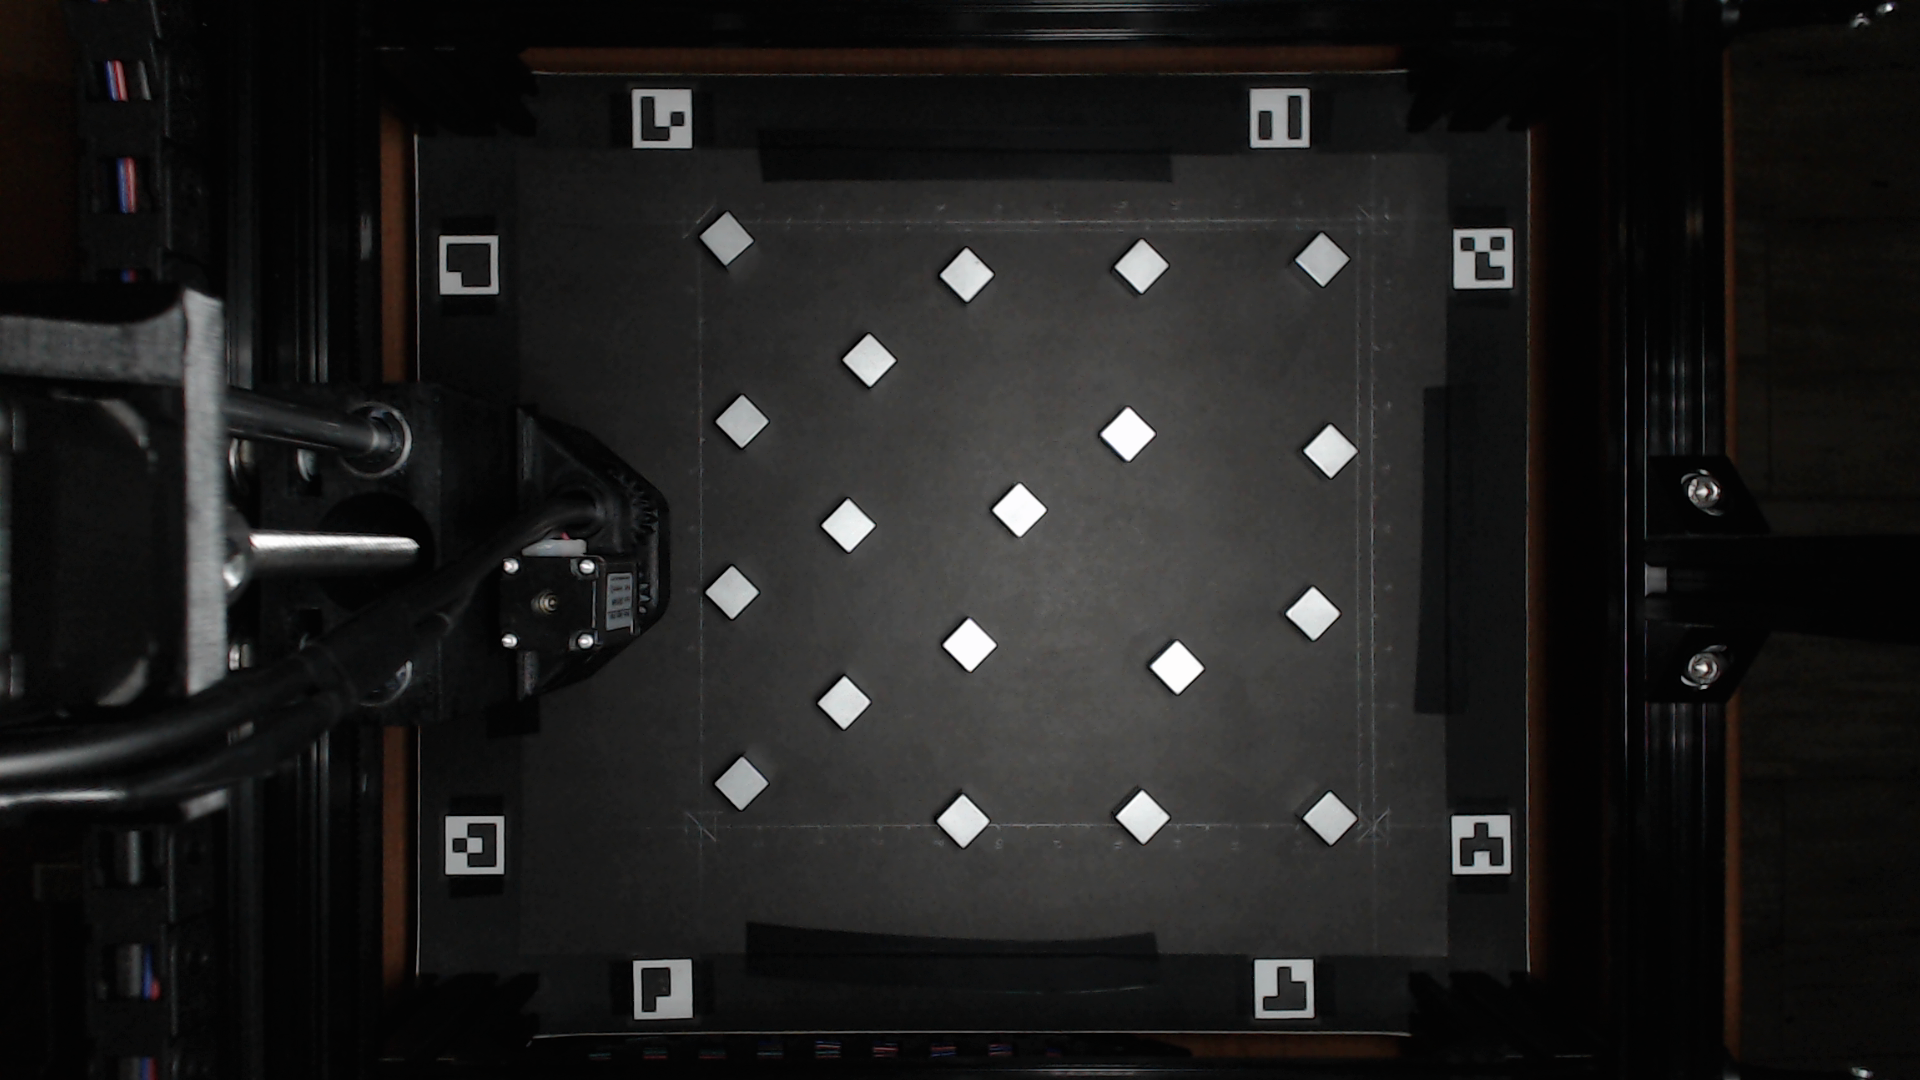
\includegraphics[width=1\linewidth]{figures/qtp6-set2.png}
	\caption{Second test set of known cube positions and orientations (45$\degree$) in the robot's workspace for qualification test 6.}
	\label{fig:qtp6-set2}
\end{figure}

\begin{figure}[!ht]
	\centering
	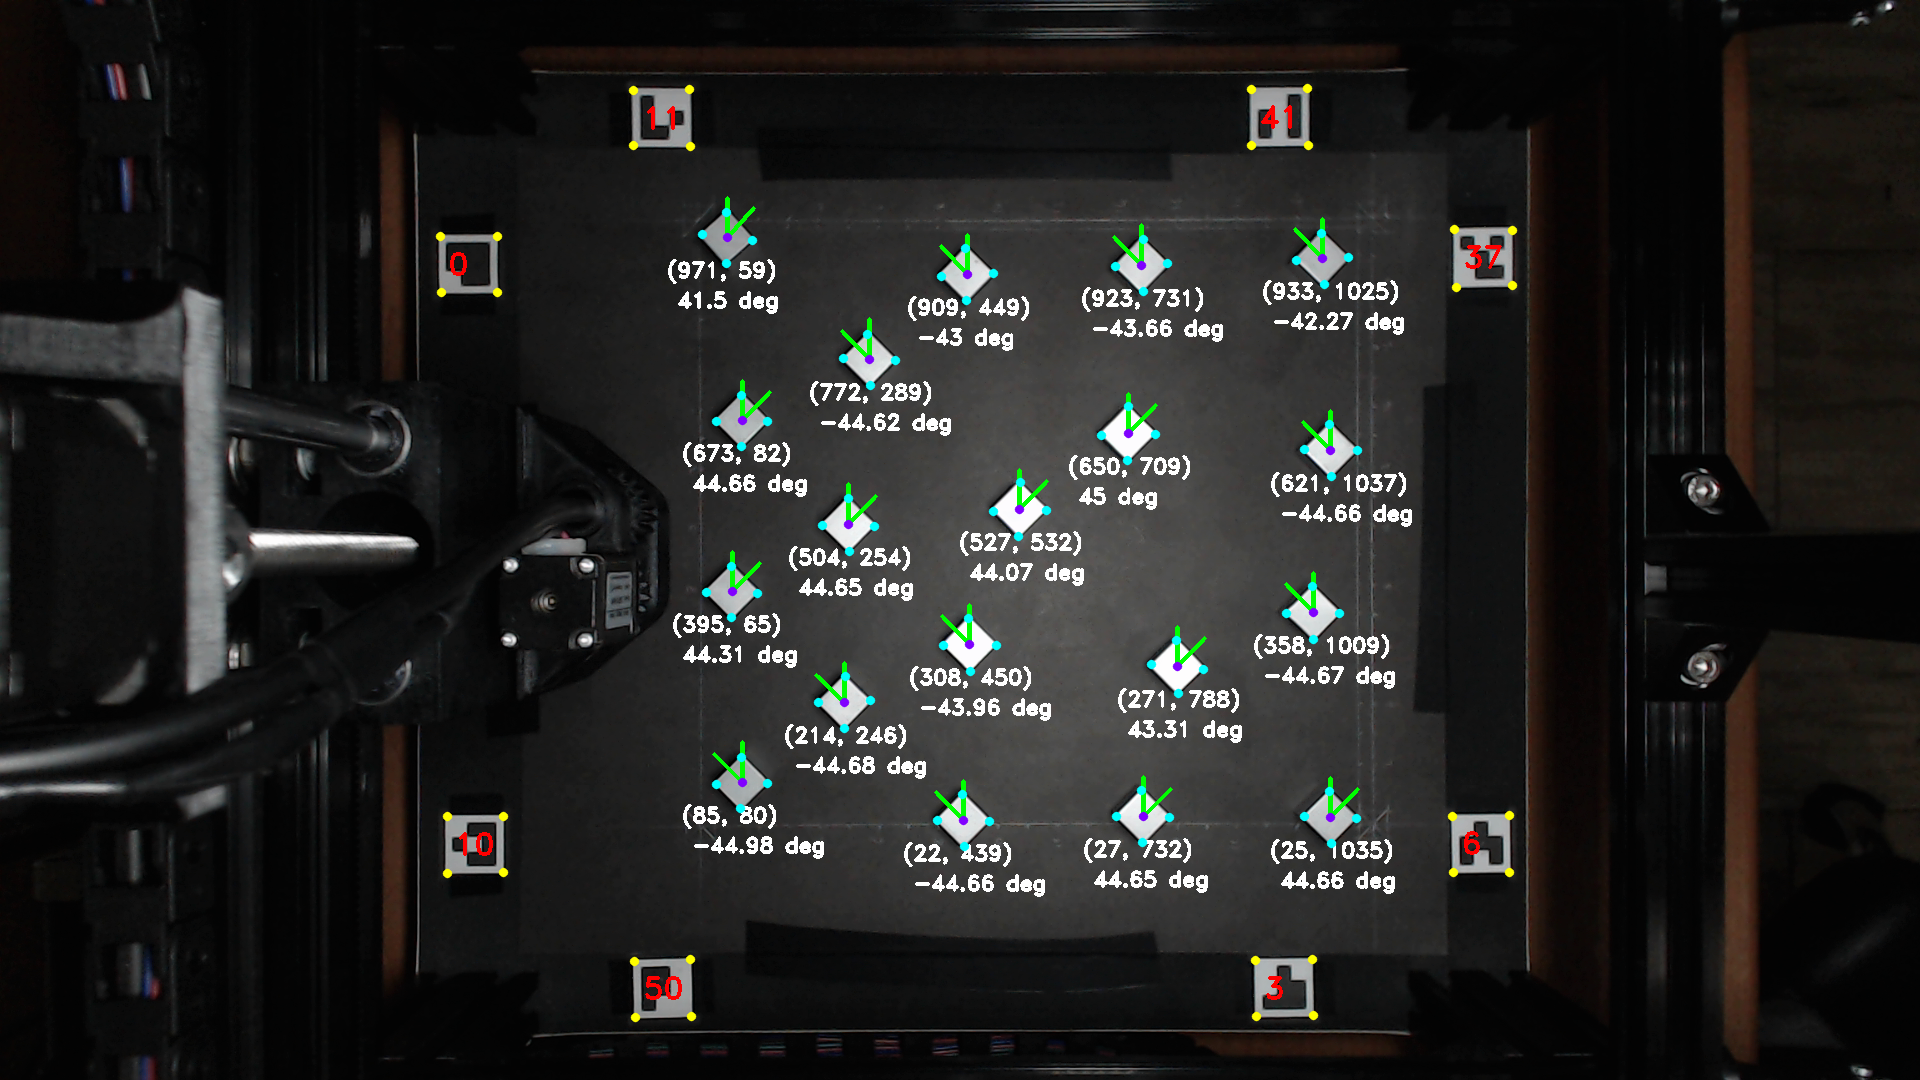
\includegraphics[width=1\linewidth]{figures/qtp6-set2-annotated.png}
	\caption{Second test set of cubes after pose estimation by the \textit{Vision System} for qualification test 6.}
	\label{fig:qtp6-set2-annotated}
\end{figure}


\subsubsecnonumhidden{Qualification Test 7 Results}

\dots



%% End of File.


